%======================================================%
%   Beamer Presentation
%   LaTeX Template
%   compile using PDFTeXify or PDFLaTeX
%======================================================%

%--------------------------------------------------------------------------------
%   PACKAGES AND THEMES
%--------------------------------------------------------------------------------

%\documentclass[notheorems,11pt,compress]{beamer}
\documentclass[notheorems,11pt]{beamer}

\setbeameroption{show notes}

\usetheme{moloch}
\usepackage{appendixnumberbeamer}

\usepackage{booktabs}
\usepackage[scale=2]{ccicons}

\usepackage{pgfplots}
\usepgfplotslibrary{dateplot}

\usepackage[english]{babel}  % Show english numerate
\molochset{block=fill}
\usepackage{xspace}
\newcommand{\themename}{\textbf{\textsc{metropolis}}\xspace}

%\usefonttheme[onlymath]{serif}
\usefonttheme{serif}
%\setbeamercovered{transparent}
%\usetheme{boxes}

%\setbeamertemplate{headline}{}
%\setbeamertemplate{footline}{}
%\setbeamertemplate{blocks}[rounded][shadow=true]
%\setbeamertemplate{blocks}[default]
\setbeamertemplate{blocks}[shadow=true]
%\setbeamercolor{block body}{bg=black!2}
\setbeamertemplate{navigation symbols}{}
%\setbeamertemplate{itemize items}[square]  % ball, circle
%\setbeamertemplate{enumerate items}[square]
%\setbeamertemplate{section in toc}[square]

\definecolor{iron}{RGB}{0,82,67}
\definecolor{footed}{rgb}{0.5,0.2,0.5}
\setbeamercolor{frametitle}{bg=iron}
%\setbeamercolor{progress bar}{fg=iron,bg=iron}

%分式使用行间版
\everymath{\displaystyle}

\setbeamertemplate{footline}
{%
\leavevmode%
%\hskip1cm \fangsong \insertshortauthor~(\insertshortinstitute) ~~\textbar~~ \insertshorttitle
\hfill\normalfont\color{footed}\insertframenumber\,/\,\inserttotalframenumber \kern1em \hfill
\vskip4pt%
}


%----------- 宏包 -------------
%\usepackage[latin1]{inputenc}
%\usepackage{times}
%\usepackage[T1]{fontenc}

\usepackage[UTF8,noindent]{ctex}
%\usepackage[english]{babel}
\usepackage{amsmath,amssymb,version}
\usepackage{graphicx,fancybox,mathrsfs,multirow}
\usepackage{booktabs}
\usepackage{epsfig,epstopdf}
\usepackage{url}
\usepackage{hyperref}
\hypersetup{
    colorlinks=true,
    linkcolor=iron,
    filecolor=magenta,      
    urlcolor=cyan,
    citecolor=blue,
}
\usepackage{tabularx,array,makecell}
\usepackage{color,xcolor}
\usepackage{cases}
\usepackage{mathtools}
\usepackage{tikz}
\usepackage{makecell}

\usepackage{scrextend}

%---------- 定义表格命令 ----------
\newcolumntype{P}[1]{>{\centering \arraybackslash}p{#1}}
\newcolumntype{L}{X}
\newcolumntype{C}{>{\centering \arraybackslash}X}
\newcolumntype{R}{>{\raggedleft \arraybackslash}X}



%---------- 设置 定理环境  --------------
\theoremstyle{plain}
\setbeamertemplate{theorems}[numbered]
%\theoremstyle{definition}
%\newtheorem{theorem}{Theorem}
\newtheorem{theorem}{定理}
\numberwithin{theorem}{section}
%\newtheorem{definition}{Definition}
\newtheorem{definition}{定义}
%\numberwithin{definition}{section}
%\newtheorem{lemma}{Lemma}
\newtheorem{lemma}{引理}
\numberwithin{lemma}{section}
%\newtheorem{proposition}{Proposition}
\newtheorem{proposition}{命题}
%\numberwithin{proposition}{section}
%\newtheorem{corollary}{Corollary}
\newtheorem{corollary}{{推论}}
\numberwithin{corollary}{section}
\theoremstyle{example}
%\newtheorem{example}{Example}
\newtheorem{example}{例}
%\numberwithin{example}{section}
\renewenvironment{proof}[1][证明]{\textbf{#1}:~}{\qed\par}
%\renewenvironment{proof}[1][证明]{{\heiti #1}:~}{\qed\par}


\setbeamerfont{caption name}{family=\rmfamily,series=\normalfont}
\setbeamertemplate{caption}[numbered]
%\numberwithin{figure}{section}
%\numberwithin{table}{section}
%\numberwithin{equation}{section}

%\addtokomafont{labelinglabel}{\normalfont}%\bfseries
%\usepackage{xunicode-addon}
%\renewfontfamily\useTIPAfont{Segoe UI}

%---------- 设置字体  ---------------
%\setbeamerfont{normal text}{family=\rmfamily}
%\setbeamerfont{frametitle}{family=\sffamily}
%\setbeamerfont{title}{family=\sffamily}
%\setbeamerfont{subtitle}{family=\sffamily}
%\setbeamerfont{institute}{family=\rmfamily}
%\setbeamerfont{author}{family=\rmfamily}
%\setbeamerfont{date}{family=\rmfamily}
%\setbeamerfont{headline}{family=\sffamily}
%\setbeamerfont{footline}{family=\rmfamily}
%\setbeamerfont{section in toc}{family=\rmfamily}
%\setbeamerfont{subsection in toc}{family=\rmfamily}
%\AtBeginDocument{\usebeamerfont{normal text}}


%---------- 定义行距 ----------
\renewcommand{\baselinestretch}{1.15}

%---------- 调节公式的间距 ----------
%\AtBeginDocument{
%	\setlength{\abovedisplayskip}{4pt plus 1pt minus 1pt}
%	\setlength{\belowdisplayskip}{4pt plus 1pt minus 1pt}
%	\setlength{\abovedisplayshortskip}{2pt}
%	\setlength{\belowdisplayshortskip}{2pt}
%	\setlength{\arraycolsep}{2pt}
%}

\makeatletter
\newcommand\HUGE{\@setfontsize\Huge{36}{42}}
\makeatother

%---------- 自定义命令 ----------
\newcommand{\red}[1]{\textcolor{red}{#1}}
\newcommand{\blue}[1]{\textcolor{blue}{#1}}


%\AtBeginSection[]{
%\begin{frame}
%  \frametitle{目录}
%  \tableofcontents[currentsection,currentsubsection]
%  %\tableofcontents[currentsection,currentsubsection,subsectionstyle=show/show/shaded]
%  \addtocounter{framenumber}{-1}
%\end{frame}
%}


%\setmonofont{Consolas}
%\setmonofont{Latin Modern Mono}
%\title{Metropolis}
%\subtitle{A modern beamer theme}
%\date{\today}
%\author{Matthias Vogelgesang}
%\institute{Center for modern beamer themes}

%----------------------------------------------------------------------------------------
%	TITLE PAGE
%----------------------------------------------------------------------------------------

\title[Short 题目]{运动规划中的混合整数规划} % The short title appears at the bottom of every slide, the full title is only on the title page

\author{汇报人：庞逸天}  % 名字
\institute[SJTU] % 机构缩写
{
上海交通大学 \\ % 机构全称
\medskip
\textit{yitianpang@sjtu.edu.cn} % 邮件
}
\date[2025.12.9]{2025~年~12~月~9~日} % 日期


\graphicspath{{./figures/}}

\begin{document}

% only change the spacing of body text
%\setlength{\baselineskip}{15pt}

\begin{frame}
\titlepage
\end{frame}

\begin{frame}{目录}
  \setbeamertemplate{section in toc}[sections numbered]
\tableofcontents
\end{frame}

%----------------------------------------------------------------------------------------
%	PRESENTATION SLIDES
%----------------------------------------------------------------------------------------

%------------------------------------------------
\section{问题背景}
%------------------------------------------------

\begin{frame}{混合整数规划}
\begin{block}{混合整数规划}
混合整数规划(Mixed Integer Programming, MIP)代表一种数学优化问题，其中目标是最小化或最大化一个线性、二次函数或有时更一般的准则，约束是线性的(或非线性的)等式(或不等式)，并且存在一些(非空)整数和实数变量子集作为参数
\end{block}
\begin{enumerate}
  \item 涉及整数的离散问题 \par
  \begin{itemize}
    \item 背包问题
  \end{itemize}
  \item 涉及逻辑条件的问题
  \begin{itemize}
    \item 复杂运输过程中的碰撞避免
  \end{itemize}
  \item 排序和分配问题
  \begin{itemize}
  \item 任务分配
  \item 旅行商问题
\end{itemize}

\note{对于离散问题，MIP通常比经典方法更好地解决问题，例如背包问题(给定一组物品，每种物品都有自己的重量和价格，在限定的总重量内，我们如何选择，才能使得物品的总价格最高).\par\vspace{1 em}
第二类适用的问题是包含逻辑条件的问题，我们稍后会介绍如何使用MIP表示逻辑条件，一个例子是碰撞避免问题，它的特点是可行区域很可能是非凸的.\par \vspace{1 em}
MIP在组合问题中较为流行，例如任务分配问题和旅行商问题，其中一个典型的例子是将航班分配到跑道上使，跑道得到高效均匀使用.其特点是它很容易拓展到图论问题，这一部分我们会在最后提及.\par}
\end{enumerate}

\end{frame}

\begin{frame}{MIP的特点与优势}
\begin{itemize}
  \item 可以非线性建模
  \item 允许非凸约束
  \item 可以包含逻辑决策
  \item 已广泛应用于控制工程问题
\end{itemize}
\note{广泛应用的控制工程问题包括：分段仿射系统辨识、分配问题、持续激励控制、混合系统控制、故障检测 或运动规划}
\end{frame}

\begin{frame}{符号与记号}
  \begin{enumerate}
    \item 逻辑运算符：$\wedge$(与), $\vee$(或), $\neg$(非)
    \item 集合的Minkowski和：$A\oplus B=\{x:x=a+b,a\in A,b\in B\}$
    \item $\|x\|^2_Q=x^TQx$
    \item 补集$C_X(S)$,闭包$\operatorname{cl}(S)$
    \item $\mathcal{V}(P)$ 表示多面体$P\subset \mathbb{R}^n$ 的(有限)顶点集
    \item $\#\mathcal{I}$表示离散集$\mathcal{I}$的基数
  \end{enumerate}
  \vspace{1 em}
  
\end{frame}

%-----------------------------------------------
\section{MIP公式化}


%-----------------------------------------------
\begin{frame}{广义析取规划(GDP)}
  \begin{exampleblock}{GDP的例子(1)}
    \begin{subequations}
    \begin{align}
      &\min_x{f(x)+\sum_k}{c_k} \\
      \text{s.t. } &r(x)\leqslant 0,x\in\mathbb{R}^n,c_k\in\mathbb{R} \\
      &\bigvee_{j\in J_k}\left[\begin{gathered}
        Y_{jk} \\
        g_{jk}(x)\leqslant 0 \\
        c_k=\gamma_{jk}
      \end{gathered}\right],k\in K \label{1c}\\
      &\Omega(Y)=\text{true},Y_{jk}\in\{\text{true,false}\} \label{1d}
    \end{align}
    \end{subequations}
  \end{exampleblock}
  \note{
    为了说明MIP对析取建模的通用性，先简要介绍GDP的相关内容.\par
    GDP旨在通过结合定量和定性信息来最优地解决化学工程问题.为此，定性信息使用析合和逻辑命题来表示.与MIP相比，GDP 方法的公式相对更紧凑，因为逻辑条件不是过布尔代数和不等式进行转换，而是以其自然逻辑形式，因此GDP代表了代数和逻辑方程的组合，例如下面的例子： \par
    $r(x)$是通用约束，不依赖于逻辑决策，$c_k$是成本变量，$\gamma_k$是固定费用，$k\in K$是析取项的数量 ，逻辑函数$\Omega(Y)$用合取范式表示. \par
    公式的逻辑是：如果$Y_{jk}$为真，那么施加约束$g_{jk}\leqslant 0$和$c_k=\gamma_{jk}$，否则忽略它们.\par
    另外，析取实际上代表了一种互斥关系，在析取$k$中，只有一个布尔变量$Y_{jk}$可以为真
  }
\end{frame}

\begin{frame}{问题1的MIP改写}
使用二元变量$y_{jk}=\{0,1\}$代替布尔变量$Y_{jk}$，并将约束(\ref{1c})替换为：
\begin{subequations}
\begin{align}
  &g_{jk}(x)\leqslant M_{jk}(1-y_{jk}) \\
  &\sum_{j\in J_k}{y_{jk}}=1,k\in K
\end{align}
\end{subequations}
其中$M_{jk}$ 是“大M”参数，为足够大的常数.\par
成本变量$c_k$看可以被重写为乘积$\gamma_{jk}y_{jk}$ ，同样地，(\ref{1d})可以重写为线性约束
$$Ay\leqslant a$$
  \note{
    上述GDP公式可以被改写为MIP形式，用二元变量代替布尔变量.\par
    (2a)代表了是之前的约束条件，当$y_{jk}=0$时，不施加约束.(2b)相当于要求了只有一个$y_{jk}$可以为真(翻页).\par \vspace{1 em}
    公式中比较重要的是大$M$参数的选取，过大的M会增加搜索域的范围，因此会增加计算量.因此我们的大M应当选取为最小的保证其不影响其他约束条件的整数，相当于一个minmax问题 \par
    GDP相对于MIP优势更小，因此现有的GDP求解器都是基于MIP重构的.但是在建模时仍然可以利用GDP建模，然后将其转化为MIP的形式即可.
  }
\end{frame}

\begin{frame}{“大M”参数的选取}
  \begin{example}
    原逻辑命题为$x>0\Longrightarrow \alpha=1$，其中$x\in\mathbb{X}=\{x:|x|\leqslant \overline{x}\}$.\par
    引入大M参数后，可将命题转化为不等式$x-M\alpha\leqslant 0$.\par
    为了使不等式满足命题的逻辑含义，需选取$M\geqslant \overline{x}$.\par
    因此最后取$M=\max_{x\in\mathbb{X}}{x}$，即$M=\overline{x}$.
  \end{example}

\end{frame}


\section{几何视角下的MIP}

\begin{frame}{多面体的半空间表示}
  \begin{proposition}{}
    有界多面体$P$都有使用半空间的交集或极限点的凸包的对偶表示$P=\{x:s_i^Tx\leqslant r_i,\forall\, i\}=\{x:x=\sum{a_jv_j,\sum{a_j}=1,a_j\geqslant 0,\forall\, j}\}$
  \end{proposition}
    \note{
    之前提到利用MIP处理的问题中可行域可能是非凸的，因此需要使用超平面排列来刻画这些非凸区域，这里介绍多面体的情形，因为大多数MIP模型的集合都是多面体，多面体有以下两种表示方式(我们在线性规划时学过的内容)(翻页) \par \vspace{1 em}
    因此超平面会把空间分成若干个不相交的区域，我们可以利用这些区域的交和并来表示所需要的区域.\par
  }
\end{frame}

\begin{frame}{多面体的半空间表示}
    基于以上命题，如果考虑来自$\mathbb{R}^d$中的有限个超平面
  \begin{equation}
    \mathcal{H}_i=\{x\in\mathbb{R}^d:h_ix=k_i\},i\in\mathcal{I}
  \end{equation}
  其中，$\mathcal{I}\triangleq \{1,\cdots,N\},(h_i,k_i)\in\mathbb{R}^{1\times d}\times\mathbb{R}$\par
  每一个超平面都会把空间分成两个不相交的区域，分别记作：
  \begin{subequations}
    \begin{gather}
    \mathcal{R}^+_i=\{x\in\mathbb{R}^d:h_ix\leqslant k_i\} \\
    \mathcal{R}^-_i=\{x\in\mathbb{R}^d:-h_ix\leqslant -k_i\}
  \end{gather}
  \end{subequations}\par
  则多面体$P$可写成这些半空间的的有界交集，另可得到其补集
  \begin{equation}
      P=\bigcap_{i\in\mathcal{I}}{\mathcal{R}^{-}_i}
  \end{equation}
  \begin{equation}
        \mathcal{C}(P)=\bigcup_{i\in\mathcal{I}}{\mathcal{R}^{+}_i} \label{6}
  \end{equation}

\end{frame}

\begin{frame}{使用二元变量表示区域}
  为了便于描述上述区域，可以引入二元变量$(\alpha_1,\alpha_N)\in\{0,1\}^N$，使用混合整数技术进行表示.\par
  \begin{subequations}
    \label{7}
    \begin{gather}
      h_ix\leqslant k_i+M\alpha_i,i\in\mathcal{I} \label{7.a}\\
      \sum_{i\in\mathcal{I}}{\alpha_i}\leqslant N-1
    \end{gather}
  \end{subequations}
  \begin{example}
    半空间$R_i^+$可以由(\ref{7.a})和以下二元变量表示：
    \begin{equation}
      (\alpha_1,\cdots,\alpha_N)=\left(1\cdots 1\;\underbrace{0}_{i}\; 1\cdots 1\right)
    \end{equation}
  \end{example}
  \note{
    如果有$N$个超平面，理论上把空间分为$2^N$个单元，可以使用二元变量组来表示这些区域.当$\alpha_i=1$时表示没有约束，反之则有约束.要求$\alpha_i$的和小于$N$的原因是当$M\to\infty$时，这种情况代表了整个$\mathbb{R}^n$.\par
    一个例子是对于一个超平面的上半空间，可以用这样的二元变量表示，也就是让$\alpha_i=0$即可.(翻页)\par \vspace{1 em}
    这种想法也可以推广到多个多面体的情形，只需要对公式稍加改写(翻页)\par \vspace{1 em}
    这一张图展示了如何选取合适的大M参数.我们的思路就是充分松弛，让它不影响其他约束，因此可以按照右式选取大M，变成了一个线性规划问题.\par
}
\end{frame}

\begin{frame}{多个多面体并集的超平面表示}
    \begin{subequations}
    \begin{gather}
      -h_{i_l}x\leqslant -k_{i_l}+M\alpha_{i_l},i\in\mathcal{I} \label{9.a}\\
      \sum_{i\in\mathcal{I}_l}{\alpha_{i_l}}\leqslant \#\mathcal{I}_l-1
    \end{gather}
  \end{subequations}
  并定义$\mathcal{I}\triangleq\bigcup_l{\mathcal{I}_l}$
\end{frame}

\begin{frame}{多面体大“M”参数的选取}
\begin{columns}[t] 
  \column{.7\textwidth} 
  \begin{figure}[h]
    \centering
    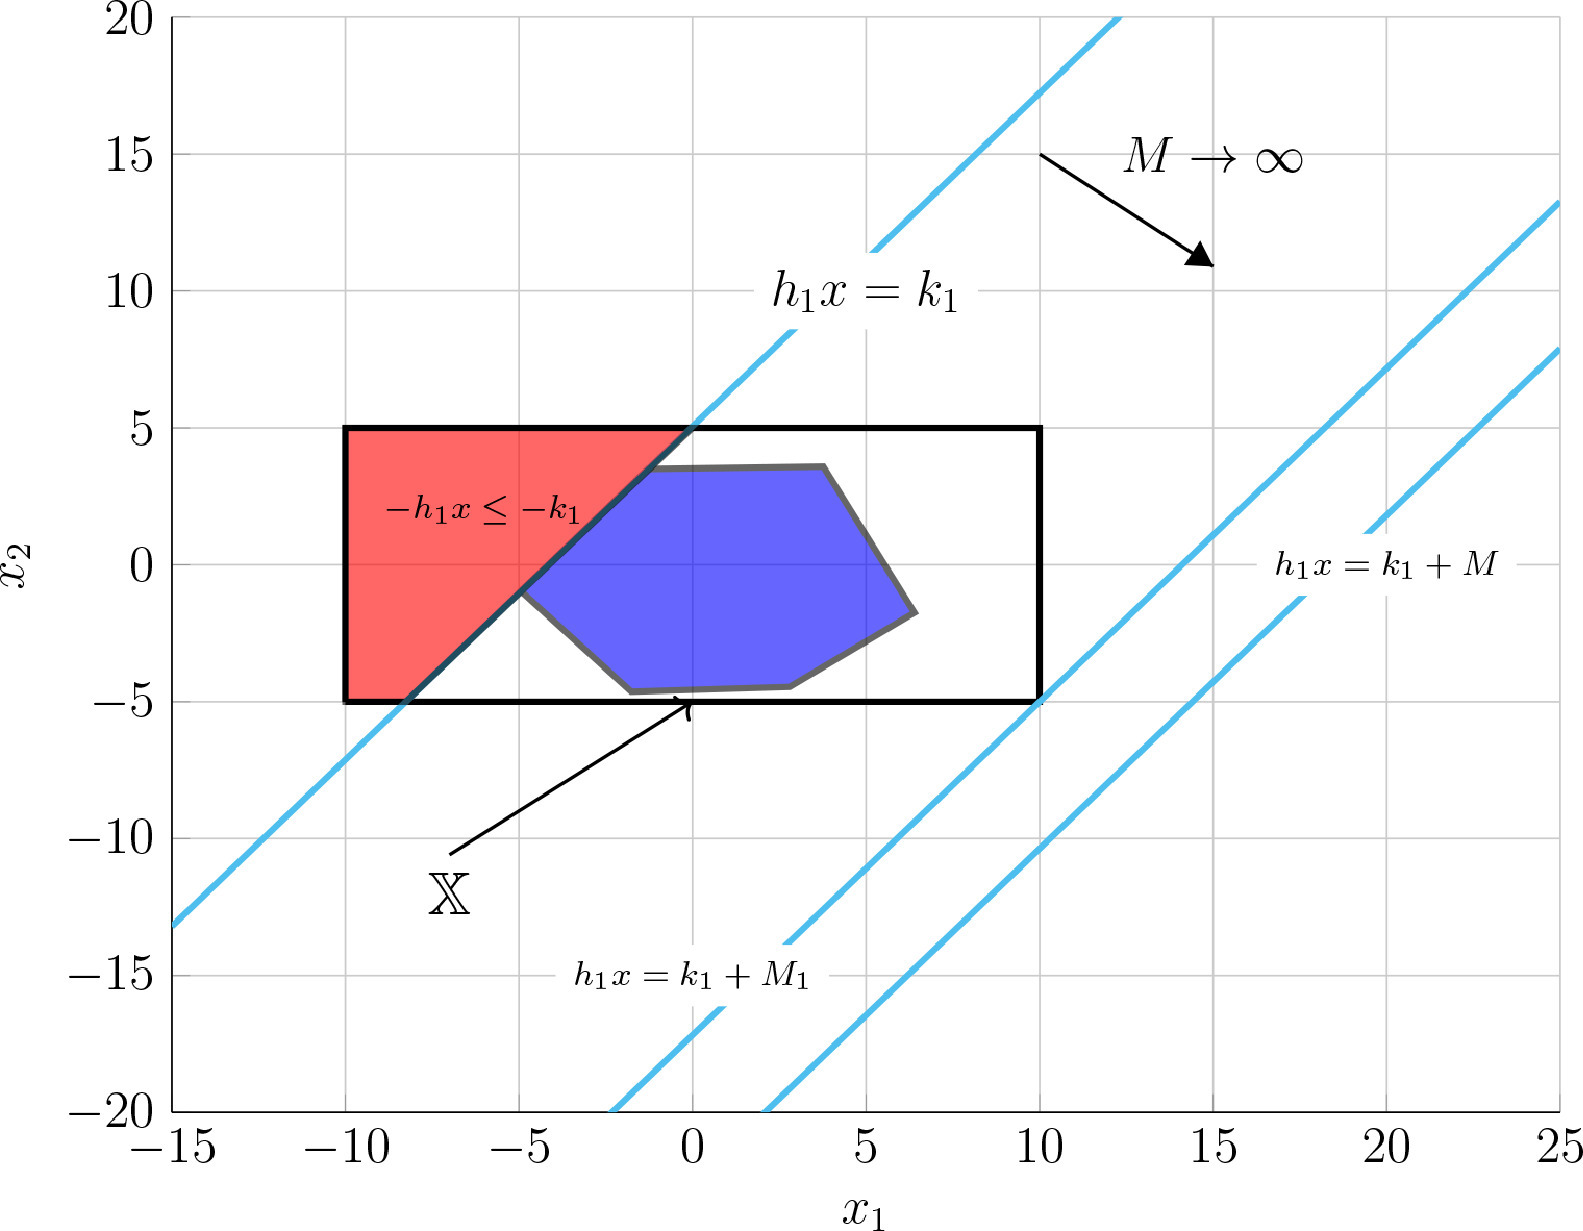
\includegraphics[width=0.95\textwidth]{fig1.jpg}
    \caption{大“M”参数选取}
    \label{fig:BigM}
  \end{figure}
  \column{.3\textwidth}
  \vspace{4.5em}
  \begin{gather*}
    M=\max_{i}M_i \\
    M_i=\max_{x\in\mathbb{X}}{(k_i-h_ix)} \\
  \end{gather*}
\end{columns}

\end{frame}


\begin{frame}{超平面排列}
  \begin{definition}[超平面排列]
    集合$\mathbb{H}$将空间划分为一系列不相交的单元$\mathcal{A}(\sigma)$，并用符号元组$\sigma\in\{-,+\}^N$表征：
    \begin{equation}
      \mathcal{A}(\sigma)=\bigcap_{i=1}^{N}{\mathcal{R}_i^{\sigma(i)}}
    \end{equation}
    覆盖全空间的单元的超平面排列由所有可行的符号元组的集合描述：
    \begin{equation}
      \mathcal{\mathbb{H}}=\bigcup_{l=1\cdots\gamma(N)}{\mathcal{A}(\sigma_l)}
    \end{equation}
    其中，$\mathbb{H}=\{\mathcal{H}_i\}_{i\in\mathcal{I}}$是半空间的非空交集产生的符号元组，$\gamma(N)$是可行单元的数量.
  \end{definition}
\end{frame}

\begin{frame}{可行域的混合整数特征}
  考虑一组障碍物
  $$\mathbb{P}=\bigcup_{j=1}^N{P_j}$$
  则可以把可行单元标记为禁止区域$\textstyle\sum_{\mathbb{P}}=\{\sigma:A(\sigma)\cap\mathbb{P}\neq\varnothing\}$和允许区域$\textstyle\sum_{X\setminus\mathbb{P}}=\{\sigma:A(\sigma)\cap\mathbb{P}=\varnothing\}$，由此得到可行域的混合整数特征：
  \begin{subequations}
    \begin{gather}
      h_ix\leqslant k_i+M(1-\alpha_i) \\
      -h_ix\leqslant -k_i+M\alpha_i \\
      \sum_{\sigma_l(i)='+'}(1-\alpha_i)+\sum_{\sigma_l(i)='-'}{\alpha_i}\geq 0\\
      \forall\,\sigma_l\in\textstyle\sum_{\mathbb{P}}
    \end{gather}
  \end{subequations}
  \note{
    当$\alpha_i=1$时，(12a)约束，(12b)松弛，此时代表了上半平面.反之则代表下半平面.(12c)保证了至少有一个符号和禁止区域不同，因此它不在禁止区域内.
    (12d)描述了禁止区域的对应的符号组.\par
    上述构建是通用的，但因为使用了二进制构造，导致复杂度是指数的，因此叶蝉生了单元和合并或对数形式化等方法降低复杂度，但如果障碍和智能体过多，仍旧可以产生不切实际的二进制变量
  }
\end{frame}

\begin{frame}{多面体障碍物}
  \begin{figure}[h]
    \centering
    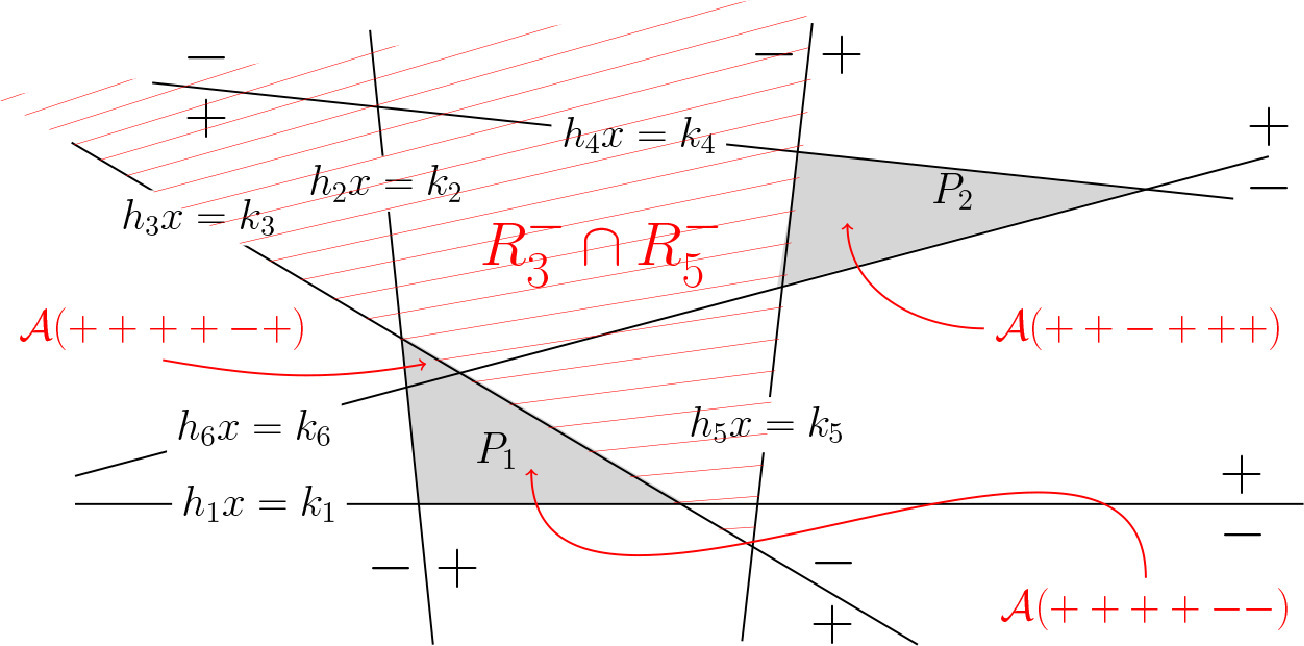
\includegraphics[width=1\textwidth]{fig2.jpg}
    \caption{多面体障碍物和超平面排列}
    \label{fig:PolyObstacle}
  \end{figure}
\end{frame}

\begin{frame}{圆形障碍物}
  \begin{figure}[h]
    \centering
    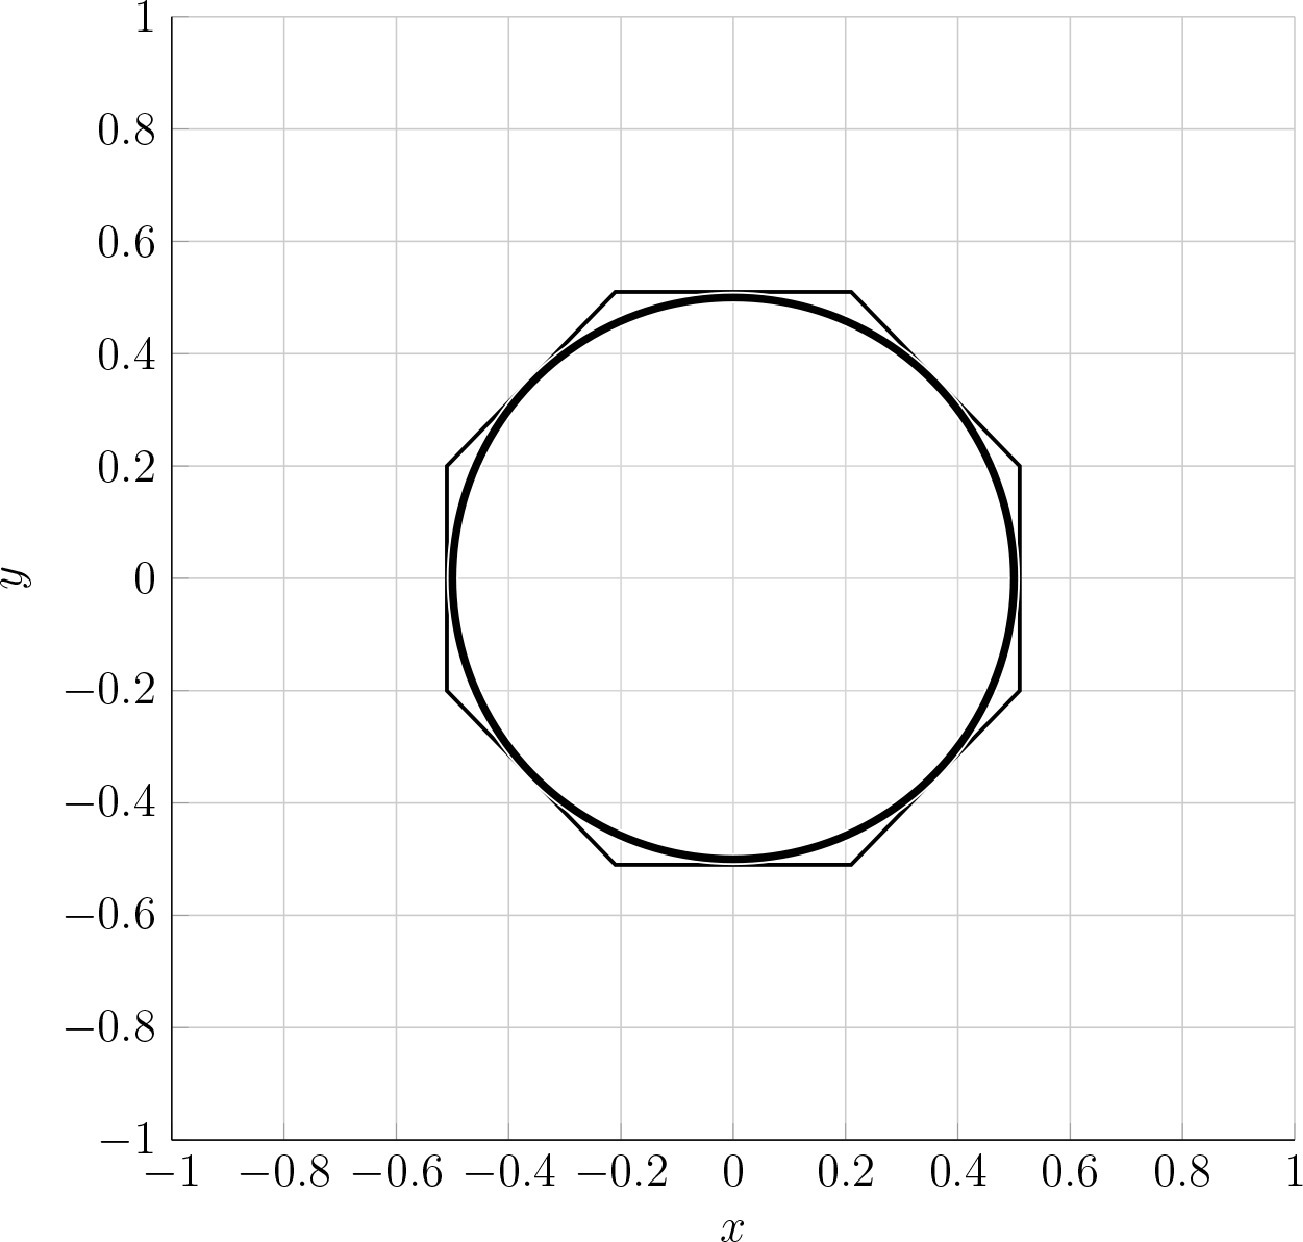
\includegraphics[width=0.5\textwidth]{fig3.jpg}
    \caption{圆形障碍物及其多面体近似}
    \label{fig:CircleObstacle}
  \end{figure}
  \begin{equation}
    \mathcal{O}=\left\{(x,y):(x-x_0)^2+(y-y_0)^2\leqslant R_0^2\right\} \label{13}
  \end{equation}
\end{frame}

\begin{frame}{圆形障碍物的混合整数表示}
  将(\ref{13})中的障碍物近似为多边形，因此每个禁止区域可以由一组$K_p$多项式描述：
    \begin{equation}
    \begin{gathered}
    \widetilde{\mathcal{O}}=\left\{(x,y):(x-x_0)\sin\frac{2\pi m}{K_p}+(y-y_0)\cos\frac{2\pi m}{K_p}\right. \\
    \left.\leqslant R_0,\forall\, m=1,\cdots,K_p\right\}
    \end{gathered}
    \end{equation}
  类似于(\ref{7})，应用混合整数技术，上述约束可以表述为：
  \begin{subequations}
    \begin{gather}
      (x-x_0)\sin\frac{2\pi m}{K_p}+(y-y_0)\cos\frac{2\pi m}{K_p}\leqslant R_0-M\beta_m,\forall\, m \\
      \sum_{m=1}^{K_p}{\beta_m}\leqslant K_p-1
    \end{gather}
  \end{subequations}
  \note{
    另外，对于非多面体的禁止区域，例如一个圆形障碍物，可以使用其多面体近似，然后再应用混合整数技术将其表示为上面得到的形式
  }
\end{frame}

\begin{frame}{使用GDP描述区域}
  考虑使用四个支撑超平面表示禁止区域，并写成GDP公式：
  对应于每个超平面$i\in\{1,2,3,4\}$，有以下析取式：
  \begin{gather*}
    \left[\begin{gathered}
      Y_{i1} \\\
      g_i(x)\leqslant 0
    \end{gathered}\right]\vee \left[\begin{gathered}
      Y_{i2} \\
      g_i(x)\geqslant 0
    \end{gathered}\right] \\
    Y_{i1}\vee Y_{i2} \leftrightarrow Y_{i2}=\lnot Y_{i1}
  \end{gather*}
  其中，$g_i(x)=x_1\pm x_2\pm 6$，并且以$Y_{i1}=\text{true}$表示$\mathcal{R}_i^-$，以$Y_{i2}=\text{true}$表示$\mathcal{R}_i^+$.
\end{frame}

\begin{frame}{GDP表示区域示例}
  \begin{figure}[h]
    \centering
    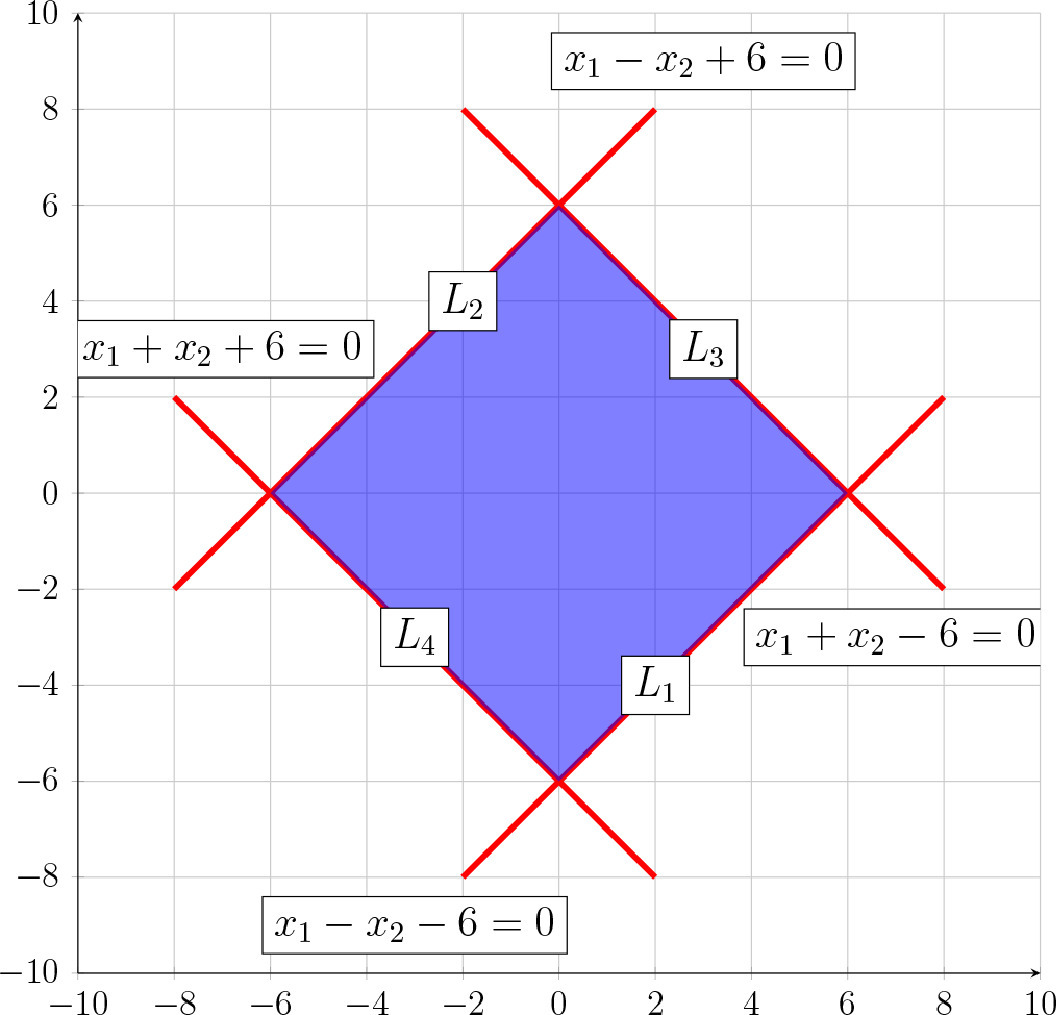
\includegraphics[width=0.4\textwidth]{fig4.jpg}
    \caption{GDP公式化示例}
    \label{fig:GDPRegion}
  \end{figure}
  \begin{gather*}
    \text{凸区域：}\Omega(Y)=\lnot Y_{11}\wedge Y_{21}\wedge \lnot Y_{31}\wedge Y_{41} \\
    \text{非凸区域：}\Omega(Y)=Y_{11}\vee \lnot Y_{21}\vee Y_{31}\vee \lnot Y_{41}
  \end{gather*}
  \note{
    这一章的最后介绍使用四个支撑超平面表示的禁止区域的GDP和MIP的表示之间的关系.\par
    我们可以利用析取式将上下平面和布尔变量联系起来，从而使用逻辑关系表示之前提到的禁止区域和允许区域.
  }
\end{frame}


%-----------------------------------------------
\section{MIP在运动规划中的应用}
%-----------------------------------------------
\begin{frame}{先决条件}
  一个由ODE描述的受控动力学系统的通用模型为：
  \begin{equation}
    \dot{x}(t)=f(x(t),u(t),w(t))
  \end{equation}
  其中，$x(t)\in\mathbb{R}^{n_x}$是状态向量，$u(t)\in\mathbb{R}^{n_u}$是控制输入向量，$w(t)\in\mathbb{R}^{n_w}$是外部扰动.映射$f(\cdot,\cdot,\cdot):\mathbb{R}^{n_x}\times\mathbb{R}^{n_u}\times\mathbb{R}^{n_w}\to\mathbb{R}^{n_x}$是一个连续函数且存在一个平衡点(即$f(\bar{x},\bar{u},0)=0$，不失一般性，假设$f(0,0,0)=0$).\par
  对应的离散动力学系统的模型为：
  \begin{equation}
    x(k+1)=f(x(k),u(k),w(k)) \label{16}
  \end{equation}
    \note{
    大部分MIP在运动规划中的应用都有一个2D或3D空间中由动力学数学模型控制的指点的动力学系统，一个通用的系统如下： \par
    同时，也有部分模型是基于离散时间动态的，因此保持相似的符号可以写出对应于离散动力学系统的模型\par 
    可以通过相应的离散化技术可以把上述两个公式联系起来(翻页)\par\vspace{1 em}
    对于线性模型和非线性模型，我们会如此选取状态向量和输入向量.\par
  }
\end{frame}

\begin{frame}{变量的选择}
  \begin{columns}[t]
  \column{.5\textwidth}
  线性模型
  \begin{itemize}
    \item 状态向量：智能体位置、速度
    \item 输入向量：智能体加速度
  \end{itemize}
  \column{.5\textwidth}
  非线性模型
  \begin{itemize}
    \item 状态向量：智能体位置、航向角
    \item 输入向量：智能体速度、转向角
  \end{itemize}
  \end{columns}

\end{frame}

\begin{frame}{最优控制问题}
  \begin{block}{最优控制问题}
    寻找一个控制输入$u^\bigstar\in\mathbb{R}^{n_u}$，使得系统(\ref{16})遵循轨迹$x^\bigstar(t)$$\in\mathbb{R}^{n_x}$，并最小化特定准则：
    \begin{subequations}
      \begin{align}
        &\min_{x(t),u(t)}J=\min_{x(t),u(t)}H \left(x(t_f)\right)+\int_{t_0}^{t_f}{L(x(t),u(t))dt}\label{18a}\\
        &\mathrm{s.t.}\; \dot{x}(t)-f(x(t),u(t),w(t))=0 \\
        &x(t_0)-x_0=0 \\
        &g \left(x(t),u(t)\right) \leqslant 0
      \end{align}
    \end{subequations}
    其中$t\in[t_0,t_f]$，$t_f-t_0$表示时间范围长度，$x_0$为初始状态，$g(\cdot,\cdot)$是一个包含物理约束的函数.
  \end{block}
  \note{
    虽然本文的重点是MIP及其实现方法，但最终获得的公式是优化控制策略的结果，因此介绍最优控制问题的概念.\par
    一个最优控制问题会根据函数$H,L$的不同选择以及时间范围的选择呈现不同的形式.\par
  }
\end{frame}

\begin{frame}{可由MIP有效解决的运动规划子领域}
  \begin{itemize}
    \item 任务分配(TA)：将一个目标分配给特定子系统的离散决策过程，其中目标可以互换且由特定准则衡量其适用性.特点是，(资源-目标)对内的方案数量可数.
    \item (无碰撞)路径规划：不显示参数化时间、不显示考虑动力学地在位置空间中构建一条路线.
    \item (无碰撞)轨迹规划：将时间与路径关联，考虑智能体动力学的特殊性，且生成的函数以开环方式产生
    \item (在线)障碍物和碰撞避免：最小化(\ref{18a})中的性能指标同时，避免碰撞且使用闭环策略寻找输入控制信号
  \end{itemize}
\end{frame}

\begin{frame}{运动规划子领域}
  \begin{figure}[h]
    \centering
    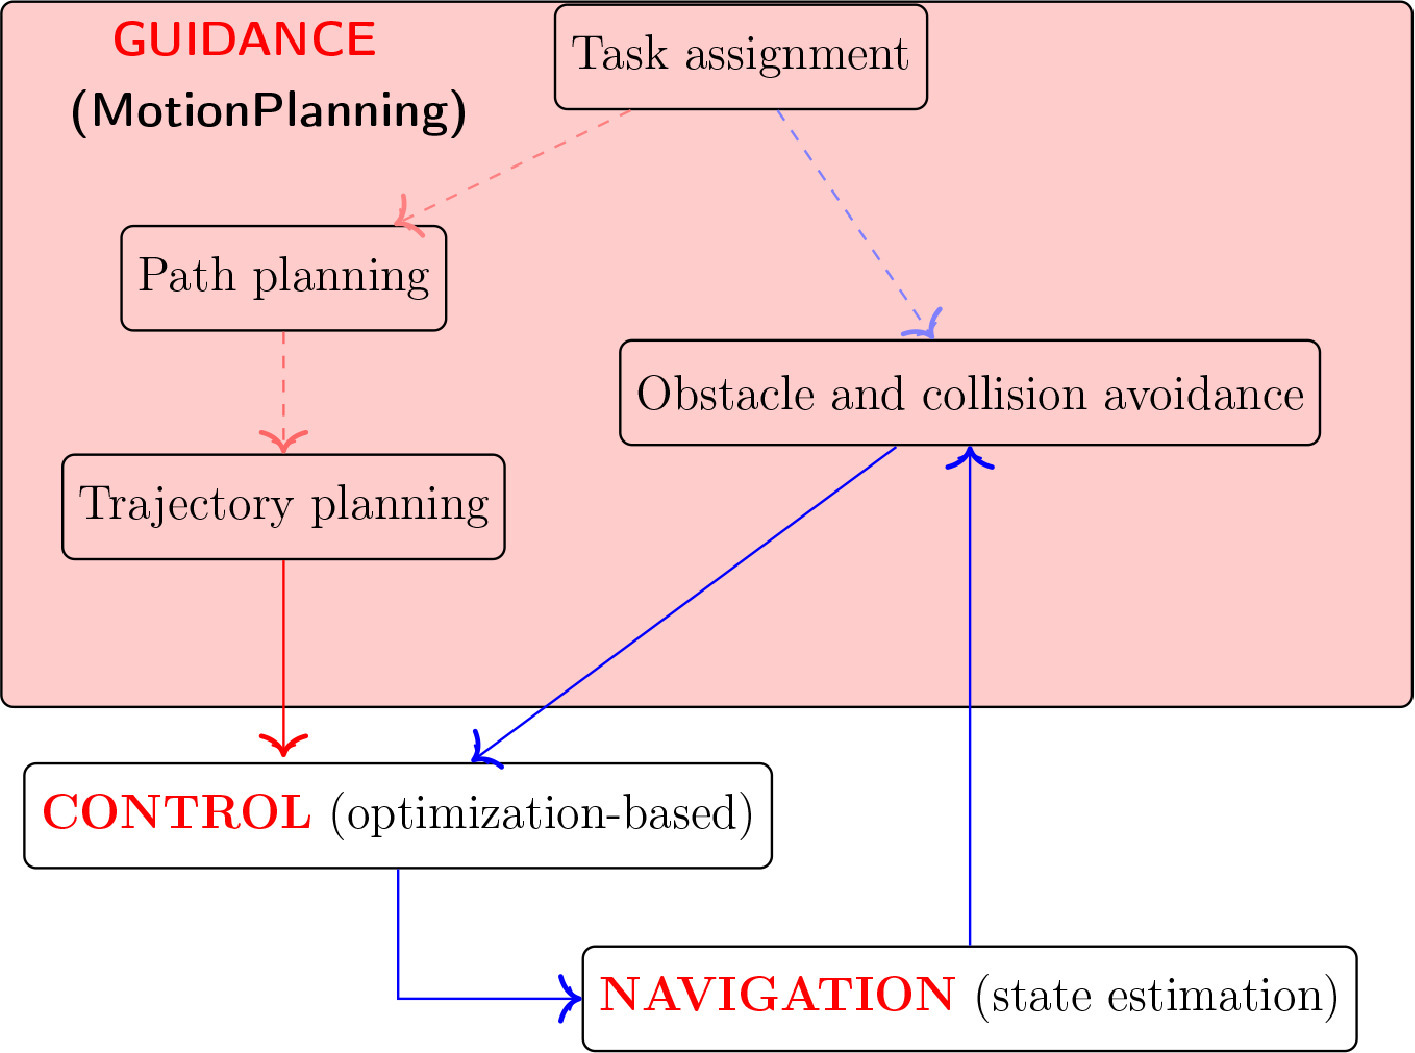
\includegraphics[width=0.8\textwidth]{fig5.jpg}
    \caption{运动规划子领域及其相互关系}
    \label{fig:MotionPlanning}
  \end{figure}
  \note{
    需要注意的时，大多数情况下，任务分配和路径规划通常不作为独立的主题处理，而是和其他子领域一起或作为其中一部分.例如路径规划通常英汉在轨迹规划中，而任务分配通常是避障或路径规划的一部分.\par
  }
\end{frame}

\begin{frame}{任务分配}
  考虑$N$个智能体和$M$个目标，需要将智能体最优地分配给目标以最小化到达所有目标的时间.定义二元变量$x_{ij}$，如果智能体$i$访问目标$j$，则$x_{ij}=1$，否则为零.另外，考虑每个智能体-目标组合成本$c_{ij}$.由此可以得到任务分配问题的标准MIP公式：
  \begin{subequations}
    \begin{align}
      &\min_{x_{ij}}\sum_{i=1}^N\sum_{j=1}^M{c_{ij}x_{ij}} \\
      &\text{s.t. } \sum_{i=1}^N{x_{ij}}\geqslant 1,\forall\, j \\
      &\sum_{j=1}^M{x_{ij}}\leqslant 1,\forall\, i \\
      &x_{ij}\in\{0,1\},\forall\, i,j \label{19d}
    \end{align}
  \end{subequations}
      \note{
    任务分配算法必须提供一个优化特定标准的分配方案，例如一场地震会影响10座建筑物，需要为每座建筑物分配一个救援队以最小化干预时间，其中需要考虑救援队的数量及它们所需的时间.\par
    更一般的，(读ppt).(19b)和(19c)限制了每个智能体必须到达一个目标以及每个目标至少要被一个智能体访问.(翻页) \par \vspace{1 em}
    上述问题属于整数线性规划的范畴，其特殊性是求解其LP松弛可以得到原来的解.但并非所有这类问题都有这一特性，例如考虑下述问题.
  }
\end{frame}

\begin{frame}{任务分配的松弛}
  使用松弛变量$X_{ij}\in [0,1]$替换(\ref{19d})并求解其LP松弛可以得到原始问题的解.\par
  但如果问题改变，例如额外定义$t_{ij}$为智能体$i$到达目标$j$的时间，并要求总时间不超过某个值(\ref{20})，则上述特性不再生效
  \begin{equation}
    \sum_{i=1}^N\sum_{j=1}^M{t_{ij}x_{ij}}\leqslant T \label{20}
  \end{equation}

\end{frame}

\begin{frame}{任务分配的变体及可以转化为MIP的问题}
  \begin{itemize}
    \item 一个智能体必须完成多个目标
    \item 无人机队列分配问题：智能体必须访问特定的航点序列
    \item 协作安全控制器：智能体分组
  \end{itemize}

  \begin{itemize}
    \item 飞机维护问题
    \item 机场调度问题
    \item 碰撞和避障问题
  \end{itemize}
  \note{
    任务分配问题还有一些变体，例如在成本中引入非线性项，对应于一个智能体必须完成多的目标.无人机队列必须访问特定的航点序列以及将智能体分组并建立相应的避障机制以防智能体之间相互威胁.\par
    另外，资源分配问题也可已被表示为MIP，由此可以处理飞机维护问题以及机场调度问题.\par
    同时，碰撞避免问题可以被视为互斥的资源分配问题，因此也可以使用MIP描述.
  }
\end{frame}

\begin{frame}{路径}
  \begin{definition}[路径]
    导航空间中两点$x_0,x_f$之间的路径由映射$\gamma:[0,1]\to \mathcal{X}$给出，其中
    \begin{equation}
      \gamma(0)=x_0,\quad \gamma(1)=x_f
    \end{equation}
  \end{definition}
  一般有两种方式描述函数$\gamma$，其一为显示方法，包括为整个区间$[0,1]$提供$\gamma$的值.其二是更常用的方法，函数必须从被称为“航点”的值中取值.\par
  定义描述规划路径的所有航点集：$\mathcal{W}=\{x_{w_0},\cdots,x_{w_{N_w}}\}$，并考虑对定义2附加条件：$\forall\, x_{w_k},\exists\, !\theta_k\in[0,1]$，使得$\gamma(\theta_k)=x_{w_k}$.
      \note{
    下面介绍路径规划和轨迹规划.这两者的差异是路径不要求显式包含时间，而轨迹必须包含时间因素，有点类似于道路和曲线的不同(翻页) \par \vspace{1 em}
    (22C)保证每个航点都被智能体访问一次，但访问航点的具体顺序取决于所选择的标准.有时候我们不要求精确抵达航点，只需要到达航点附近，则可以对(22b)进行松弛.
  }
\end{frame}

\begin{frame}{路径规划}
  处理路径规划问题的常用方法是将其转化为旅行商问题(TSP).
  \begin{example}[Richards,How(2002)、Schouwenaars(2006)]
    考虑一个需要访问$N_w$个航点的机器人，同时最小化操作成本，因此，强制访问所考虑航点的MI约束如下：
    \begin{subequations}
      \begin{gather}
        \forall\, i\in\{1,\cdots,T\},\forall\, k\in\{1,\cdots,N_w\}, \\
        \|x_i-x_{w_k}\|\leqslant M(1-b_{ik}) \\
        \sum_{i=1}^T{b_{ik}}=1,\forall\, k\,\text{且}\, b_{ik}\in\{0,1\} \label{22c}
      \end{gather}
    \end{subequations}
    其中$T$是时间步的数量，$b_{ik}$是二元变量，表示在时间步$i$时是否访问了航点$k$.约束(\ref{22c})确保机器人访问每个航点一次
  \end{example}

\end{frame}

\begin{frame}{路径规划的其他方法}
  \begin{itemize}
    \item Tunnel-MILP方法
    \begin{enumerate}
      \item 忽略车的动力学约束，找到一条路径
      \item 该路径与空间的凸分解形成从起点到目标的一系列$N_R$个凸多面体$F_i=\{x\in\mathbb{R}^2:A_ix\leqslant b_i\}$
      \item 使用多面体隧道将智能体$p(t)$的位置约束在隧道内从起点到目标的最佳动态可行道路上
      \begin{equation}
      \bigvee_{i\in\{1,\cdots,N_R\}}{A_ip(t)\leqslant b_i},\forall\, t
    \end{equation}
    \end{enumerate}
      \note{
    除了上述方法，路径规划还有一些其他方式.(读ppt)\par
    它使用了一个MILP问题，迫使智能体始终保持在隧道的某个区域，从而可以使用MI技术表示如下：(翻页)\par \vspace{1 em}
    另外可以使用详细的思想，使用广义Voronoi图来寻找路径
  }
  \end{itemize}

\end{frame}

\begin{frame}{路径规划的其他方法}
  \begin{itemize}
    \item 广义Voronoi图
    \begin{enumerate}
      \item 通过障碍物的面和导航环境的边界构建广义Voronoi图
      \item 移除禁止区域内的节点与连接这些节点的边
      \item 使用Delaunary三角剖分将空间划分为三角形，并计算被规划路径穿过的三角形，将其合并形成多图面体，试图隧道中的凸区域数量最少
    \end{enumerate}
  \end{itemize}

\end{frame}

\begin{frame}{轨迹}
  \begin{definition}[轨迹]
    导航空间中两个店$x_0,x_f$之间的轨迹由连续函数$\gamma:[t_0,t_f]\to \mathcal{X}$给出，其中
    \begin{equation}
      \gamma(t_0)=x_0,\quad \gamma(t_f)=x_f
    \end{equation}
  \end{definition}
  类似于路径，轨迹也通常有连续函数和航点集表示两种方式指定.对于第二种方式，描述轨迹的所有航点集修改如下：$\widetilde{\mathcal{W}}=\left\{\left(x_{w_0},t_{w_0}\right),\cdots,\left(x_{w_{N_w}},t_{w_{N_w}}\right)\right\}$.
\end{frame}

\begin{frame}{各种任务中的轨迹规划}
  \begin{itemize}
    \item Earl和D'Andrea(2005a)：提出一种迭代MILP算法，可以保证车辆在轨迹上保证避开圆形障碍物，且有效分配避障时间.
    \item Earl和D'Andrea(2002)：利用混合系统对机器人的简化比赛进行建模，将其转化为一个MLD系统，并可以使用最先进的MILP求解器求解
    \item Cetin、Bikdash和Hadaegh(2007)：解决了航天器编队重构生成无碰撞轨迹，且实现最佳燃油消耗.使用三次样条将轨迹在时间上离散化，并使用大“M”方法将参数化优化写成MILP，并使用求解器求解
    \item Richards和How(2003)：使用MILP进行开环车辆轨迹设计，从而可以包含非凸约束，例如避免羽流撞击
  \end{itemize}
\end{frame}

\begin{frame}{自动驾驶任务中的轨迹规划}
  \begin{itemize}
    \item Molinari(2017)：为自主超车问题引入了一种高效的MIP公式.考虑的车辆具有简单动力学模型，并用超平面排列表示非凸可行区域.针对被多个智能体围绕的情况，提出了生成避免碰撞的轨迹的未完整模型，在IPG CarMaker中得到验证
    \item Ballesteros-Tolosana(2017)：针对确保乘客舒适度的变道和超车操作的轨迹生成问题这一OCP问题，使用多重shooting方法求解枚举所有超车配置及其产生的紧凑型MIP公式，计算负担有所改进.
  \end{itemize}
\end{frame}

\begin{frame}{自动驾驶任务中的轨迹规划}
  \begin{itemize}
    \item Fayazi(2017)：目标是找到车辆穿过交叉路口最优序列及其访问时间，最小化当前时间和最后通过交叉口的到达时间差异与每辆车分配访问时间和期望访问时间之间的差距.通过MIP建模，将总优化成本由一个min-max问题和含有绝对值的非线性成本组成.
    \item 黄和彭(2017)：优化交叉口的车辆速度轨迹，最小化燃油消耗和行驶时间.假设已知交通信号且忽略前车影响，考虑交叉口的转弯情况，提出一个MIP公式，用整数变量模拟了激活的绿灯时段.
    \item 张、苏、孙、张(2017b)：提出了判断一个交叉路口是否需要信号控制的方法
    \item 张、苏、高、张(2017a)：提出了考虑车辆和行人后的交通信号调度策略，被称述为MIQP问题.
  \end{itemize}
\end{frame}

\begin{frame}{障碍物和碰撞避免}
  \begin{block}{障碍物和碰撞避免}
    障碍物和碰撞避免问题是指在最小化(\ref{18a})中性能指标的同时，通过闭环策略避免碰撞，找到输入控制信号的问题.
  \end{block}
  \begin{enumerate}
    \item 选择一种不依赖于环境特定细节的划分方法，将碰撞避免问题转化为资源分配问题
    \item 使用集合论和混合整数技术有效编码非凸集
  \end{enumerate}
\end{frame}

\begin{frame}{静态障碍物}
  \begin{itemize}
    \item Culligan(2006)：使用MILP解决了无人机的递推预测控制优化问题，包括障碍物和多车辆规避的硬约束和车辆动力学近似，并全面考虑3D情况.
    \item Schouwenaars(2006)：采用MPC框架提出了一种用于无人驾驶车辆在部分未知环境中完全在线轨迹规划的框架.其可以同时通过标准速度控制系统或允许从一组可能的动作中选一个实现控制.
    \item Maia、Galvao(2009)，Richards、Turnball(2013)：考虑额外约束确保两个连续位置之间不会穿过障碍物
    \item Stoican，Prodan和Grotli(2018)：在超平面排列设置中对多障碍物情况进行处理，使用了精确以及近似的表示
  \end{itemize}
\end{frame}

\begin{frame}{移动障碍物}
  在二维环境中两个移动障碍物的MIP公式中的禁止区域约束如下：
  \begin{subequations}
    \begin{gather}
      x_1-x_2\geqslant d-M\alpha_{d1} \\
      x_2-x_1\geqslant d-M\alpha_{d2} \\
      y_1-y_2\geqslant d-M\alpha_{d3} \\
      y_2-y_1\geqslant d-M\alpha_{d4} \\
      \sum_{i=1}^4{\alpha_{di}}\leqslant 3
    \end{gather}
  \end{subequations}
  其中，$d$是安全距离，$\alpha_{di}$是二元变量.
\end{frame}

\begin{frame}{避障问题在自动驾驶车辆中的应用}
\begin{itemize}
  \item Mukai,Natori,Fujita(2017)：使用MIP和滚动时域策略解决高速公路车辆的并道问题
  \item Molinari(2017)：使用滚动时域策略处理自动超车问题，其中车辆具有简单的动力学模型
  \item Bali和Richards(2018)：基于滚动时域策略，采用MIQP优化，提出了一种用于交叉路口车辆并道场景的方法，在保证安全性和递归可行性的同时，提供了最优控制特性.
\end{itemize}
\end{frame}

\begin{frame}{混合动力学系统}
  混合动力学系统(MLD)为建模和控制包含线性动力学方程、逻辑规则和操作约束的系统提供了通用框架，系统由线性动力学方程描述，并受涉及实数和整数变量的线性不等式约束：
  \begin{subequations}
    \begin{gather}
      x_{k+1}=Ax_k+Bu_k+B_2\delta_k+B_3z_k \label{26a}\\
      y_k=Cx_k+Du_k+D_2\delta_k+D_3z_k \\
      E_2z_k+E_3\delta_k\leqslant E_1u_k+E_4x_k+E_5
    \end{gather}
  \end{subequations}
  其中，$x_k,y_k,u_k$分别表示系统的状态、输出和输入变量，$\delta_k\in\{0,1\}^{n_\delta}$和$z_k\in\mathbb{R}^{n_a}$是辅助逻辑变量和连续变量.
\end{frame}

\begin{frame}{避障的MLD等效公式}
  考虑单个智能体表述的系统，并需要在非凸域内移动，智能体的动力学方程为
  \begin{subequations}
    \begin{gather}
      x_{k+1}=Ax_k+Bu_k \label{27a}\\
      y_k=Cx_k+Du_k \label{27b}
    \end{gather}
  \end{subequations}
  要求智能体必须停留在多面体外部$\begin{aligned}
    &P=\{x:Sx<R\} \\
    &x_{k+1}\notin P
  \end{aligned}$
\end{frame}

\begin{frame}{避障的MLD等效公式}
  将$B_2,B_3$视作零矩阵，则(\ref{27a})与(\ref{26a})等价，接下来，根据动力学替换$x_{k+1}$，有
  \begin{equation}
    \left[\begin{gathered}
      -MI_N \\
      \mathbf{1}^T
    \end{gathered}\right]\alpha_k\leqslant \left[\begin{gathered}
      SA \\
      \mathbf{0}
    \end{gathered}\right]x_k+\left[\begin{gathered}
      SB \\
      \mathbf{0}
    \end{gathered}\right]u_k+\left[\begin{gathered}
      -R \\
      N-1
    \end{gathered}\right] 
  \end{equation}
  其中$N$是描述多面体$P$的线性约束的数量，再通过对输入$(S_uu_k\leqslant R_u)$添加约束，最终的MLD公式为
  \begin{subequations}
  \begin{gather}
    x_{k+1}=Ax_k+Bu_k \label{29a}\\
    \left[\begin{gathered}
      -MI_N \\
      \mathbf{1}^T \\
      \mathbf{0}
    \end{gathered}\right]\alpha_k\leqslant \left[\begin{gathered}
      SA \\
      \mathbf{0} \\
      \mathbf{0}
    \end{gathered}\right]x_k+\left[\begin{gathered}
      SB \\
      \mathbf{0} \\
      -S_u
    \end{gathered}\right]u_k+\left[\begin{gathered}
      -R \\
      N-1 \\
      R_u
    \end{gathered}\right]
  \end{gather}
  \end{subequations}
\end{frame}

\begin{frame}{漂移抵消最优控制的MIP重构}
  \begin{block}{漂移抵消最优控制}
    漂移抵消最优控制(DCOC)是一种特殊的最优控制问题，旨在确定一系列控制输入，以最大化从给定集合的首次退出时间
  \end{block}
  \begin{itemize}
    \item Zidek(2017)：在航天器姿态控制中讨论了DCOC的MILP形式，并引入了一种基于LP的迭代过程求解
    \item Maia、Galvao(2009)：提出一种用于MPC控制器的移位预测视界实现
    \item Richards、How(2003)：使用MILP优化实现可变视界长度
  \end{itemize}
\end{frame}


%------------------------------------------------
\section{多智能体系统中的MIP\\连通性维护和编队控制}
%------------------------------------------------

\begin{frame}{连通性维护和编队控制}
  \begin{block}{连通性维护}
    连通性维护通常指反馈律、路径/轨迹规划、避障和任务分配的集合，以保证智能体之间可以相互通信.
  \end{block}
  \begin{block}{编队控制}
    编队控制旨在提供约束，以保证一组智能体之间期望的相对距离和速度.
  \end{block}
  \begin{enumerate}
    \item 领导者-跟随者方法：指定一个智能体作为领导者以特地你给凡是移动，其余智能体跟踪领导者在其周围保持编队
    \item 无领导者方法：通过全局共识协调智能体以实现全局目标
  \end{enumerate}
\end{frame}

\begin{frame}{拐角切割避让条件}
  \begin{block}{拐角切割}
    当且仅当智能体的下一个位置位于其可见区域内时，智能体才避免拐角切割.\par
    可见区域是从当前位置出发的所有不与任何障碍物相交的射线的并集
  \end{block}
  由于难以精确描述此类区域，因此使用混合整数公式描述，具体使用三个符号三元组：智能体的当前和未来的位置$\sigma,\sigma^+\in \textstyle\sum_{X\setminus\mathbb{P}}$，以及障碍物的坐标$\sigma^*\in\textstyle\sum_{\mathbb{P}}$.
\end{frame}

\begin{frame}{Maia,Galvao(2009)}
  为了避免切割单个障碍物，必须存在至少一个包含该障碍物的半空间，且该半空间不包含智能体的当前和后继位置：
  \begin{equation}
    \exists\, i,\mathrm{s.t.}\; \sigma(i)=\sigma^+(i)=0 \label{30}
  \end{equation}
  此类问题常出现在MPC问题，其中符号元组都是决策变量，因此可以被重写以避免非线性：
  \begin{equation}
    \sum_{i}[1-\sigma^\circ(i)]\sigma^+(i)<N+\sum_{i}[1-2\sigma^\circ(i)]\sigma(i) \label{31}
  \end{equation}
  对于所有可能的$\sigma^\circ\in\{0,1\}^N$，至少有一个约束(\ref{31})会被简化为(\ref{30})，即当$\sigma^\circ=\sigma^+$
\end{frame}

\begin{frame}{Richards,Turnball(2015)}
  改进了上述约束，将约束(\ref{31})的$2^N$个约束减少为$N$个.强制两个连续位置$x,x^T$遵守相同的约束：
  \begin{gather*}
    -h_i^Tx\leqslant -k_i+M\sigma^+(i) \\
    -h_i^Tx^+\leqslant -k_i+M\sigma^+(i) \\
  \end{gather*}
  则对所有$i=1,2\cdots,N$，至少一个$i$使得$x,x^+$在超平面的同一侧.\par
  更进一步，Afonso等人(2016)提出了对数方案，减少了选择活动超平面时涉及的二进制变量的数量.
\end{frame}

\begin{frame}{Stoican(2018)}
  \begin{equation}
    \sum_{i=1}{|\sigma^{\bullet,j}(i)-\sigma(i)|\cdot|\sigma^{\bullet,j}(i)-\sigma^+(i)|}>0,\forall\,\sigma^{\bullet,j}\in\textstyle_{\mathbb{P}} \label{32}
  \end{equation}
  当$\sigma,\sigma^+$都是变量时，同样可以使用(\ref{31})中的松弛方法
  \begin{equation}
    \sum_{i=1}{|\sigma^{\bullet,j}(i)-\sigma^\circ(i)|\cdot|\sigma^{\bullet,j}(i)-\sigma^+(i)|}>-|\sigma^\circ-\sigma|,\forall\,\sigma^{\bullet,j}\in\textstyle_{\mathbb{P}} \label{33}
  \end{equation}
  当$\sigma^\circ=\sigma^+$时，(\ref{33})简化为(\ref{32}).
\end{frame}

\begin{frame}{连通性维护条件}
  混合整数约束要求每个智能体至少与另一个智能体在通信范围内，同时避免配对孤立(即一个智能体被强制留在另一个智能体的通信范围内时，后者不能被约束在前者的通信范围内).考虑二元变量$\xi_{i,j,k}\in\{0,1\}$，当$i$号智能体在时间步$k$时位于$j$号智能体的通信范围内时，变量为1,否则为0，则连通性维护条件为：
  \begin{subequations}
    \begin{gather}
      \sum_{i=1}^{N-1}\sum_{j=1}^N\xi_{i,j,k}=N-1,0\leqslant k\leqslant T \\
      \sum_{v_i,v_j}\xi_{i,j,k}\leqslant \# S-1,0\leqslant k\leqslant T,\forall\, S\subset V \\
      \xi_{i,j,k}=0,1\leqslant i\leqslant N,1\leqslant j\leqslant i,0\leqslant k\leqslant T 
    \end{gather}
  \end{subequations}
\end{frame}

\begin{frame}{由外部约束引起的连通性}
  最为典型的示例是移动传感器对特定区域进行有效覆盖的问题.\par
  \vspace{1 em}
  Ritter等人(2014)通过由一组配备传感器的自主车辆组成的移动传感器平台解决了该问题魔提出了一种自适应观测策略.\par
  该策略基于过程模拟和多带沥血做系统，使用MLD系统建模，并用PDE估计代理的目标位置.
\end{frame}


%------------------------------------------------
\section{控制架构}
%------------------------------------------------
\begin{frame}{控制架构的分类}
  \centering
  \begin{tabular}{|c|c|c|}
    \hline
    控制架构 & 特点 & 优点与缺点  \\
    \hline
    集中式 & \makecell[c]{多智能体系统视为整体\\物理系统被完全忽略\\可以使用单个全局控制器} & \makecell{理论简单、常用\\扩展系统复杂引发数值困难}\\ 
    \hline
    分布式 & \makecell[c]{全局问题划分为子问题\\子问题涉及局部控制器\\智能体无法访问全局信息} & \makecell{复杂性与可扩展性降低\\稳定性和鲁棒性降低}\\
    \hline
    去中心化 & \makecell[c]{全局问题划分为子问题\\智能体有一个控制器\\不考虑其他智能体行为\\信息交换受限} & \makecell{潜在的高效策略\\无法保证最优性}\\
    \hline
  \end{tabular}
\end{frame}

\begin{frame}{集中式控制架构的应用}
  \begin{itemize}
    \item Chen等人(2016a)：考虑$N$个具相似动态特性的智能体，每个智能体由保证其完成目标的活性控制器和远离其他智能体的危险区域的安全控制器.后者使用了集中式架构，保证了$N=3$时的情况.MIP用于提供高级逻辑.
    \item 对于全局场景，所有智能体掌握彼此动态，因此可以使用非凸约束实现碰撞避障
    \item Wang(2015)：研究了多智能体系统中的碰撞避免，将碰撞避免问题转化为了资源分配问题，使用MIP解决相关优化问题.
  \end{itemize}
\end{frame}

\begin{frame}{分布式控制架构的应用}
  \begin{itemize}
    \item Schouwenaars(2006)：采用分布式MPC策略导航车队穿越部分位置和杂乱的环境
    \item Testa,Rucco,Notarstefano(2017)：提出了用于求解MILP的算法，约束分布在各个智能体之间
    \item Mariéthoz, and Morari (2016)：基于拉格朗日对偶，提出了对大规模MILP特别有效的分解办法
    \item Van Parys and Pipeleers (2016)：使用交替方向乘子法构建问题
  \end{itemize}
\end{frame}

\begin{frame}{去中心化控制架构的应用}
  \begin{itemize}
    \item BaliandRichards(2018)：提出了合并交叉路口问题，根据定义的标准对多个到达交叉路口的智能体进行有限级排序
  \end{itemize}
\end{frame}





%------------------------------------------------
\section{使用MIP的控制软件}
%------------------------------------------------

\begin{frame}{MIP实现的软件示例}
\begin{table}[htbp]
    \centering
    % \resizebox{宽度}{高度}{内容}
    % \textwidth 表示适应页面宽度，"!" 表示高度自动按比例缩放
    \resizebox{\textwidth}{!}{
        \begin{tabular}{|c|c|c|}
        \hline
        \multicolumn{2}{|c|}{\textbf{软件}} & \textbf{参考文献 (例如)} \\ \hline
        \multirow{3}{*}{编程语言} & MATLAB & Bemporad and Mignone (2000); Culligan (2006); Janeček et al. (2017a) \\ \cline{2-3} 
         & Python & Welder et al. (2018) \\ \cline{2-3} 
         & Julia & Lubin, Yamangil, Bent, and Vielma (2018) \\ \hline
        \multirow{7}{*}{建模语言} & Yalmip & Mukai et al. (2017); Zhang et al. (2017b) \\ \cline{2-3} 
         & GAMS & Lee and Grossmann (2000) \\ \cline{2-3} 
         & CVX/ & Dueri et al. (2017) \\ \cline{2-3} 
         & CVXPY &  \\ \cline{2-3} 
         & Pyomo & Legg et al. (2012) \\ \cline{2-3} 
         & JuMP & Welder et al. (2018) \\ \cline{2-3} 
         & AMPL & Richards and How (2005, 2002) \\ \hline
        \multirow{3}{*}{求解器} & CPLEX & Janeček et al. (2017a); Stoican et al. (2013) \\ \cline{2-3} 
         & GUROBI & Janeček et al. (2017a) \\ \cline{2-3} 
         & SCIP & Berthold et al. (2012) \\ \hline
        \end{tabular}
    }
    \end{table}
\end{frame}

\begin{frame}{MIP求解方法和启发式技术}

    \begin{table}[htbp]
    \centering
    % 使用 resizebox 自动缩放表格宽度以适应页面
    \resizebox{\textwidth}{!}{
        \begin{tabular}{|c|c|}
        \hline
        \textbf{求解方法} & \textbf{参考文献} \\ \hline
        分支定界法 & Bemporad (2015); Bemporad and Mignone (2000); \\ \hline
        变体 & \makecell{Bemporad et al. (1999); Feng et al. (2017);\\ Hespanhol et al. (2019); Naik and Bemporad (2017)} \\ \hline
        ADMM & \makecell{Abboud et al. (2015); Kanno and Kitayama (2018);\\ Scott and Thiébaux (2014); Takapoui et al. (2020);\\ Timotheou et al. (2014)} \\ \hline
       FP & \makecell{Fischetti et al. (2005); Fischetti and Salvagnin (2009); \\ Miertoiu and Dumitrescu (2019)} \\ \hline
        \end{tabular}
    }
    \end{table}

\end{frame}

\begin{frame}{启发式算法简介}
  \begin{itemize}
    \item ADMN:常用于最优功率流问题.Stellato，Naik,Bemporad，Goulart和Boyd(2018) 开发了一种新颖的分支定界算法，专门为基于ADMM的求解器量身定制
    \item FP：用于寻找给定MIP可行解的启发式算法，旨在最小化LP松弛解与原始MIP解之间的差异.Miertoiu和Dumi-trescu(2019)改变该算法用于稀疏表示
  \end{itemize}
\end{frame}

\begin{frame}{硬件平台}

    \begin{table}[htbp]
    \centering
    % 这里的 0.2\textwidth 和 0.75\textwidth 分别代表列宽占页面宽度的比例
    % 可以根据需要调整，总和最好不要超过 1.0
    \resizebox{\textwidth}{!}{
        \begin{tabular}{p{0.2\textwidth} p{0.75\textwidth}}
        \toprule[1.5pt] % 顶部粗线
        \textbf{实验平台} & \textbf{参考文献} \\
        \midrule % 中间细线
        
        \textbf{无人机} & Bellingham 等人 (2002a, 2002b); Chen 等人 (2016a); \newline
                        Culligan (2006); Papen 等人 (2017); Ragi 和 Mittelmann \newline
                        (2017); Rey 和 Hijazi (2017); Richards 和 How (2002); \newline
                        Schouwenaars (2006) \\ 
                        
        \vspace{1ex} % 增加一点行间距，让两个条目分得更开
        
        \textbf{无人地面车辆} & Bali 和 Richards (2018); Ballesteros-Tolosana 等人 \newline
                        (2017); Fayazi 等人 (2017); Molinari 等人 (2017) \\ 
                        
        \bottomrule[1.5pt] % 底部粗线
        \end{tabular}
    }
    \end{table}
\end{frame}


%------------------------------------------------
\section{MIP的替代方案}
%------------------------------------------------

\begin{frame}{MIP的替代方案}
  \begin{table}[htbp]
    \centering
    % \resizebox{宽度}{高度}{内容}
    % \textwidth 表示适应页面宽度，"!" 表示高度自动按比例缩放
    \resizebox{\textwidth}{!}{
    \begin{tabular}{|c|c|}
        \hline
        \textbf{方法/技术} & {\textbf{参考文献}} \\ \hline
        
        基于图的算法 & 
        \makecell{Hsu 等人 (2007); Karaman 和 Frazzoli (2011);\\ Ladd 和 Kavraki (2004); LaValle (2006);\\ Lozano-Pérez 和 Wesley;Weiss 等人 (2017)} \\ \hline
        
         势场公式 & 
        \makecell{ Chen 和 Wang (2005); Filotheou 等人 (2018); \\ Rimon 和 Koditschek (1992); Vlantis, Vrohidis, Bechlioulis 和 Kyriakopoulos (2018);\\ Vrohidis, Vlantis, Bechlioulis 和 Kyriakopoulos (2018)} \\ \hline
        
        凸松弛 & 
        \makecell{Liu 和 Lu (2014); Mao 等人 (2017, 2016) \\Harris 和 Açıkmese (2014), Rey 和 Hijazi (2017) \\Frasch 等人 (2013); Janeček 等人 (2017a);\\ Yu 等人 (2014)} \\ \hline
    \end{tabular}}
    \end{table}
\end{frame}

\begin{frame}{基于图的算法}
  该算法将离散决策简化为搜索图中节点的最短路径，可应用于任何基于MIP的运动规划问题.
  \begin{enumerate}
    \item 考虑环境的显示表示，基于单元分解构建图.无碰撞路径是智能体在初始位置和最终位置之间通过该图的最短路径.
    \item 基于采样，避免显示表达环境以缓解计算负担，重点被放在碰撞检测上
    \begin{itemize}
      \item PRM：一种多查询方法，构建线路图后通过计算图中的最优路径回答查询
      \item RRT：更适用于环境未知的场景，图的构建和路径搜索同时进行，得到的图是树状的
    \end{itemize}
  \end{enumerate}
\end{frame}

\begin{frame}{基于图的算法与其他控制策略结合}
  \begin{itemize}
    \item Berntorp, Danielson, Weiss, 和 Di Cairano (2018)：使用反馈控制、正不变集和闭环系统的平衡轨迹提出了一种实时集成运动规划方法
    \item Altché和Fortelle(2017)：通过一种将可行区域分区的方法来解决轨迹规划问题，转化为二次凸目标函数优化问题
    \item Franzè和Lucia(2015)：处理了未知环境中避障问题
  \end{itemize}
\end{frame}

\begin{frame}{势场公式}
  势场公式通过给成本中添加罚函数来添加约束.它依赖于构造一个标量函数，使得当智能体停留在禁止区域时，函数取告知，以此使函数沿势的负梯度方向移动到最终点.
\end{frame}

\begin{frame}{凸松弛}
  \begin{block}{凸松弛}
    将非凸公式转化为凸公式，且不会产生任何重大差距，被称为凸松弛或非凸优化问题的凸化.常见的凸化方法例如：凸松弛、连续凸化或时变约束.
  \end{block}
\end{frame}

\begin{frame}{连续凸化}
  连续凸化的基本思想是通过一系列凸子问题解决非凸最优控制问题.\par
  针对于来自非线性动力学或非凸约束的非凸性，都是用线性化来处理，通常使用一阶泰勒展开近似.
  \begin{itemize}
    \item Dueri、Mao、Mian、Ding和Açikmeşe(2017)：使用连续凸化技术处理了在包含圆柱形和椭圆形障碍物的环境中自动驾驶汽车的非凸轨迹优化问题.再过程中，为了缓解近似误差和人为不可行性，作者又分别引入了信任域和惩罚函数
  \end{itemize}
\end{frame}

\begin{frame}{时变约束}
  将非凸域分解为一系列凸区域，并引入切换时刻.在每个时刻，智能体都应停留在某个凸区域内.\par
  时变约束可以视作连续凸化的特例，区别在于获得凸子问题/子域序列的方式。时变约束方法考虑了先验已知的子域数量，而连续凸化是一种迭代方法，序列会不断增长直到获得可行解.
\end{frame}

\begin{frame}{其他的凸松弛}
  \begin{itemize}
    \item Rey和Hijazi(2017):，提出了一种不同的凸松弛方法，公式基于复数表示，并为本质上非凸的优化问题提供了紧密的凸松弛.这种方法在Coffrin、Hijazi和Hentenryck(2017)中得到了广泛处理，其中通过导出相应的凸包来处理非凸约束，问题被转化为MIQCP(混合整数二次约束规划)
    \item Huang和Peng(2017)：使用顺序凸优化方法(即通过形成凸子问题来搜索局部最优解)来解决MI 优化问题
    \item Papen等人(2017)：使用约束松弛和调整复杂度来限制计算时间，从而解决了MILP问题
  \end{itemize}
\end{frame}

\section{总结与未来挑战}

\begin{frame}{未来挑战}
  \begin{enumerate}
    \item 碰撞避免问题的大规模问题仍具有较大的复杂性，无法实时求解
    \item 求解算法有待调整改进，适应问题的不同特性以降低混合整数方法的固有复杂性
    \item 基于MIP的运动规划中的工作很少能在实验平台上验证理论结果
  \end{enumerate}
\end{frame}



\end{document}


